%---------- Quarto Capítulo: Desenvolvimento ----------

\chapter{Desenvolvimento} %10 --- 20 pags

\section{Ferramentas Utilizadas}
\subsection{Sistema Operacional}

O desenvolvimento deste projeto foi totalmente realizado em ambiente Linux, em diferentes distribuições derivadas do Debian: Ubuntu 12.04 e Xubuntu 11.10.

\subsection{Ambientes de Desenvolvimento Integrado}

A primeira etapa de desenvolvimento planejada foi a de construir um modelo para a nova interface gráfica. Tendo em vista a linguagem Java como requisito, optou-se pelo \sigla{IDE}{Integrated Development Environment} NetBeans (versão 7.1.1) que possui uma ferramenta nativa específica para a construção de interfaces gráficas para usuário, a \sigla{GUI}{Graphical User Interface} Builder (Graphical User Interface). Esta ferramenta permite a construção de formulários no estilo drag-and-drop de containers existentes no Java, como por exemplo JFrame, JPanel, JButton, etc.

Inicialmente, o IDE Eclipse também foi utilizado com a finalidade de se realizar modificações nos projetos originais model e service. Posteriormente, para unificar o projeto em apenas um ambiente de desenvolvimento, os projetos originais foram importados no NetBeans.

\subsection{Outras ferramentas}

Os códigos em C++ foram desenvolvidos através do editor de textos Vim, um editor de textos gratuito e de código aberto amplamente configurável para permitir edições eficientes de texto \cite{vimabout}. Este editor é uma versão aperfeiçoada do editor Vi, presente na maioria dos sistemas \sigla{UNIX}{Sistema Operacional}.

Para criar executáveis dos códigos C++ gerados, foi utilizado o compilador g++. Este compilador faz parte da coleção de compiladores \sigla{GCC}{GNU Compiler Collection} \cite{gccabout} produzida e mantida pelo \sigla{GNU Project}{Projeto de desenvolvimento de software livre} \cite{gnuabout}.

A fim de automatizar o processo de geração de executáveis, a ferramenta \emph{make} foi configurada de acordo. Esta ferramenta, também mantida pelo GNU Project, permite que vários códigos-fonte sejam processados ao mesmo tempo através de um arquivo de configuração chamado \emph{makefile}, que pode executar um compilador para gerar arquivos-objeto, ou executar um \emph{linker} para gerar executáveis \cite{makeabout}.
 
\subsection{Controle de Versões}

Em função de a equipe contar com dois integrantes desenvolvedores, existe a necessidade de se utilizar uma ferramenta para o controle de versões do projeto. Primeiramente, para realizar testes de algumas funcionalidades foi preciso modificar radicalmente o código o que, em certos casos, não gerou resultados satisfatórios, sendo necessário retornar à um ponto estável e funcional. Além deste motivo, o sistema de controle de versões escolhido, o Git, possui ferramentas de resolução de conflitos eficientes que auxiliam o desenvolvimento simultâneo.

O Git é um software livre e gratuito distribuído sob a licença \sigla{GNU}{General Public License} General Public License versão 2 \cite{git}.

Aliado a esta ferramenta, foi utilizado um serviço web de hospedagem de projetos que é organizado pelo sistema de controle de versões Git, o GitHub cujo endereço é http://github.com. Existem funcionalidades no estilo rede social como feeds, seguidores e gráficos diversos, bem como funcionalidades de projeto como visualização de pastas e códigos, gráficos de desempenho por usuário, por equipe, por período de desenvolvimento, frequência de código, histórico de modificações, entre outros \cite{githubabout}.

Na versão gratuita, que foi a utilizada, há uma exigência: que o código seja aberto \cite{githubabout}. Na versão paga, existem planos que permitem a criação de repositórios privados com times de desenvolvimento. Para ambas as versões o número de colaboradores é ilimitado, assim como o número de repositórios públicos.

\section{Ferramentas Desenvolvidas}
\label{des:ferramentas}

As ferramentas foram planejadas para uma utilização modular, ou seja, para serem utilizadas através da \emph{interface} do SASQV assim como através da linha de comando, de forma independente. Um dos requisitos destas ferramentas é a de que sejam aplicadas sobre vídeos no formato YUV com subamostragem 4:2:0 \emph{progressive}.

\subsection{Raffle}
\label{des:raffle}

A ferramenta raffle tem como objetivo gerar elementos aleatórios multi-dimensionais no domínio dos naturais, armazenado-os em arquivo.

No arquivo gerado, cada coluna representa uma dimensão que deve seguir alguma distribuição de probabilidade, informada via parâmetros. Dentre as distribuições possíveis e seus respectivos parâmetros tem-se: 

\begin{itemize}
	\item Distribuição constante: a dimensão correspondente terá valor constante c para todos os elementos gerados.
	\item Distribuição uniforme: a dimensão correspondente terá valores uniformemente gerados num intervalo [a, b).
	\item Distribuição normal: a dimensão correspondente terá valores gerados conforme uma distribuição normal, de média m e desvio padrão d.
	\item Distribuição triangular: a dimensão correspondente terá valores gerados conforme uma distribuição triangular no intervalo [a, b) com pico em c.
\end{itemize}

A Tabela \ref{tab:distparam} sintetiza os parâmetros que devem ser informados conforme o tipo de distribuição desejada.

\begin{table}[!h]
	\centering
	\caption{Distribuições e respectivos parâmetros para a execução da ferramenta raffle.}
	\label{tab:distparam}
	\begin{tabular}{l|l|l|l|l}
		\hline
		Distribuição & \multicolumn{4}{c}{Parâmetros} \\
		\hline
		Constante  & -d ou -u & constant   & -p ou -r & a \\
		Uniforme   & -d ou -u & uniform	   & -p ou -r & a,b \\
		Normal     & -d ou -u & normal	   & -p ou -r & m,d \\
		Triangular & -d ou -u & triangular & -p ou -r & a,b,c \\
		\hline
	\end{tabular}
\end{table}

Adicionalmente aos parâmetros de cada distribuição, a primeira coluna possui uma característica temporal que pode ser ativada, permitindo a repetição de determinado elemento ao longo de um intervalo constante ou aleatório. Para este sorteio é possível utilizar qualquer distribuição descrita acima.

O comando para utilizar a ferramenta e seus parâmetros são descritos a seguir:

\begin{table}[!h]
	\begin{tabular}{llll}
	./raffle & & \\ 
	& \texttt{--output} & \texttt{-o} & arquivo\_de\_saída \\
	& \texttt{--durationdist} & \texttt{-u}  & tipo de distribuição da duração \\
	& \texttt{--durationparams} & \texttt{-r}  & parâmetros da distribuição da duração \\
	& \texttt{--elements} & \texttt{-e}  & elementos a serem gerados \\
	& \texttt{--dist} & \texttt{-d}  & tipo de distribuição da primeira dimensão \\
	& \texttt{--params} & \texttt{-p}  & parâmetros da distribuição da primeira dimensão \\
	& ... & \\
	& \texttt{--dist} & \texttt{-d}  & tipo de distribuição da n-ésima dimensão \\
	& \texttt{--params} & \texttt{-p}  & parâmetros da distribuição da n-ésima dimensão \\
	& \texttt{--help} & \texttt{-h}  & menu de ajuda \\
	\end{tabular}
\end{table}

Observações:
\begin{itemize}
    \item[-] Todo parâmetro -d deve ser imediatamente sucedido por um parâmetro -p
    \item[-] O parâmetro -u deve ser imediatamente sucedido por um parâmetro -r
    \item[-] Cada conjunto (-d -p) representa uma dimensão, ou uma coluna, a ser gerada.
\end{itemize}

Exemplos de utilização através da linha de comando são descritos abaixo. A diferença para a \emph{interface} gráfica reside apenas no fornecimento dos dados, uma vez que a \emph{interface} deve executar o mesmo comando para gerar o arquivo.

No comando a seguir, será gerado um arquivo com nome raffleout.rff contendo 30 elementos. Para este exemplo, será utilizado um valor de duração constante e igual a 1, no próximo exemplo este conceito de duração será melhor detalhado. A primeira dimensão deve seguir uma distribuição uniforme dentro do intervalo [1, 5), a segunda dimensão deve ter valor constante 3 para todos os elementos gerados e a terceira e última dimensão deve seguir uma distribuição triangular no intervalo [3, 20) com pico no ponto 10.

./raffle -o raffleout.rff -u constant -r 1 -e 30 -d uniform -p 1,5 -d constant -p 3 -d triangular -p 3,20,10

O resultado de uma execução deste comando pode ser observado na Tabela \ref{tab:raffleresult1}, a seguir:

\begin{table}[!h]
	\centering
	\caption{Resultado de execução do commando raffle para exemplo 1.}
	\label{tab:raffleresult1}
	\begin{tabular}{|l|l|l|l|l|l|}
		\hline
		4 3 6 & 1 3 16 & 1 3 16 & 1 3 18 & 3 3 16 & 3 3 11 \\
		3 3 18 & 3 3 11 & 2 3 6 & 2 3 13 & 2 3 10 & 3 3 14 \\
		1 3 11 & 2 3 11 & 4 3 9 & 4 3 11 & 2 3 15 & 3 3 10 \\
		1 3 9 & 3 3 11 & 2 3 7 & 1 3 7 & 4 3 5 & 1 3 4 \\
		1 3 10 & 3 3 11 & 4 3 10 & 4 3 11 & 2 3 12 & 3 3 6 \\
		\hline
	\end{tabular}
\end{table}

No comando abaixo, será gerado um arquivo de nome raffleout2.rff com 50 elementos de duas dimensões: a primeira seguirá uma distribuição uniforme dentro do intervalo [1,5) e a segunda seguirá uma distribuição normal com média 2 e desvio padrão 1:

./raffle -o raffleout2.rff -u constant -r 3 -e 50 -d uniform -p 1,5 -d normal -p 2,1

A duração, neste exemplo, tem duração constante 3, ou seja, para todo elemento gerado, ele deverá ter duração de 3 elementos no total. O efeito da duração pode ser observado na figura, onde o primeiro elemento (4 1) tem duração 3 tendo a primeira dimensão como referência temporal: (4 1), (5 1) e (6 1). A geração de elementos prossegue até que o número de elementos gerados atinja o desejado, informado no parâmetro -e. Um resultado importante, que pode ser observado na Tabela \ref{tab:raffleresult2}, é que a duração não ultrapassa os limites definidos para a primeira coluna fazendo com que nem todos os artefatos tenham a duração estabelecida.

\begin{table}[!h]
	\centering
	\caption{Resultado de execução do commando raffle para exemplo 2.}
	\label{tab:raffleresult2}
	\begin{tabular}{|l|l|l|l|l|l|l|l|l|l|}
		\hline
		3 2 & 4 2 & 3 1 & 4 1 & 4 1 & 2 1 & 3 1 & 4 1 & 3 2 & 4 2 \\
		3 4 & 4 4 & 2 3 & 3 3 & 4 3 & 4 1 & 1 2 & 2 2 & 3 2 & 4 1 \\
		4 0 & 3 2 & 4 2 & 3 1 & 4 1 & 4 1 & 2 3 & 3 3 & 4 3 & 1 2 \\
		2 2 & 3 2 & 1 0 & 2 0 & 3 0 & 1 2 & 2 2 & 3 2 & 2 2 & 3 2 \\
		4 2 & 2 3 & 3 3 & 4 3 & 1 0 & 2 0 & 3 0 & 1 2 & 2 2 & 3 2 \\
		\hline
	\end{tabular}
\end{table}

%TODO
Na aplicação do efeito de blocagem, por exemplo, a posição de cada pixel no vídeo é representada por uma tupla de três dimensões: o frame F em que o pixel aparece, a posição X em relação ao eixo vertical e a posição Y em relação ao eixo horizontal. Na simulação de rede, os vídeos são representados por uma sequência de pacotes,

A ferramenta raffle foi inicialmente utilizada de forma interna nas ferramentas block e netsim. %TODO

\subsection{Block}

Esta ferramenta é responsável por aplicar o efeito de blocagem sobre o vídeo desejado. Os parâmetros que devem ser fornecidos são descritos a seguir:

\begin{table}[!h]
	\begin{tabular}{llll}
	./block & & \\ 
	& \texttt{--input} & \texttt{-i}  & arquivo\_de\_entrada \\
	& \texttt{--output} & \texttt{-o}  & arquivo\_de\_saída \\
	& \texttt{--size} & \texttt{-s}  & dimensões do vídeo de entrada no formato WxH \\ 
	& & & (largura por altura em pixels) \\
	& \texttt{--window} & \texttt{-w}  & tamanho da janela da \sigla{DCT}{Discrete Cosine Transform} \\
	& \texttt{--levelsdct} & \texttt{-l}  & níveis DCT à serem eliminados, separados por vírgulas \\
	& \texttt{--rafflelist} & \texttt{-r}  & arquivo\_raffle \\
	& \texttt{--help} & \texttt{-h}  & menu de ajuda \\
	\end{tabular}
\end{table}

A partir do vídeo desejado, deve-se escolher o nome do vídeo resultante e informar as dimensões do vídeo original, o tamanho da janela a ser utilizada na DCT, os subníveis de energia que deverão ser eliminados (zerados) e o nome do arquivo raffle a ser utilizado.

O arquivo raffle de entrada deve sempre conter três colunas. A primeira diz respeito ao \emph{frame} em que será aplicado o artefato. A segunda e a terceira coluna devem ter como limite o resultado da divisão da largura e altura do vídeo pelo tamanho da janela desejada, respectivamente, pois seus valores indicam qual grupo de pixels será afetado e nao o pixel inicial de aplicação da DCT.

Os subníveis de energia (diagonais da matriz resultante da DCT) que serão cancelados dependem diretamente do tamanho da janela a ser aplicada. Seja uma janela de dimensões AxA, existem N = 2A-1 níveis de energia. O maior nível, 2A-1, representa o nível de energia \sigla{DC}{Differential Coding} (\emph{Differential Coding}) (a média dos valores do bloco). Nos demais níveis, conforme o nível diminui, a energia diminui porém a frequência aumenta. São conhecidos como coeficientes \sigla{AC}{Arithmetic Coding} (\emph{Arithmetic Coding}). A Figura \ref{fig:niveisdct} apresenta a organização dos níveis de energia numa janela de dimensões 8x8 pixels.

\begin{figure}[!htb]
	\centering
	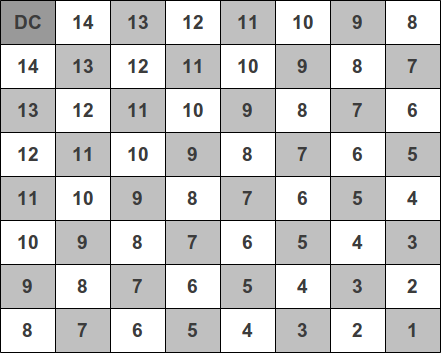
\includegraphics[width=0.5\textwidth]{./imgs/niveisdct.png}
	\caption{Diagonais de energia do bloco DCT.}
	\label{fig:niveisdct}
	\fonte{\cite{}}
\end{figure}

O arquivo gerado deve ter as mesmas características do original: tamanho em bytes, largura e altura.

Como exemplo de utilização temos que na execução do comando a seguir, o arquivo saida.yuv de dimensões 352x288 será gerado. O vídeo original será submetido aos valores contidos no arquivo raffle\_352x288.rff e cada janela de dimensões 8x8 terá os níveis DCT (ou diagonais) 1,2,4,6,7,15 zerados.

./block -i entrada.yuv -o saida.yuv -s 352x288 -w 8 -l 1,2,4,6,7,15 -r raffle\_352x288.rff

A única restrição se deve aos valores do arquivo raffle, como já mencionado. Este deve conter três colunas, em que a primeira, segunda e terceira colunas devem ter como limites superiores, respectivamente, o número de \emph{frames} do vídeo original e as dimensões largura e altura divididas pelo tamanho da janela (352/8 = 44 e 288/8 = 36).

\subsection{Blur}

A ferramenta blur aplica o artefato de borramento utilizando para tanto um filtro da média ou um filtro da mediana, de dimensão configurável. O arquivo de saída é gerado aplicando-se o artefato configurado em todos os frames do vídeo original. Os parâmetros de configuração e respectivas descrições podem ser observados adiante:

\begin{table}[!h]
	\begin{tabular}{llll}
	./blur & & \\ 
	& \texttt{--input} & \texttt{-i}  & arquivo\_de\_entrada \\
	& \texttt{--output} & \texttt{-o}  & arquivo\_de\_saída \\
	& \texttt{--size} & \texttt{-s}  & dimensões do vídeo de entrada no formato WxH \\ 
	& & & (largura por altura em pixels) \\
	& \texttt{--blur} & \texttt{-b}  & tipo do filtro a ser aplicado \\
	& \texttt{--window} & \texttt{-w}  & tamanho do filtro \\
	& \texttt{--help} & \texttt{-h}  & menu de ajuda \\
	\end{tabular}
\end{table}

Numa possível execução da ferramenta como indicada abaixo, o filtro da média de dimensões 5x5 pixels será aplicado no vídeo original, gerando o vídeo degradado saida.yuv de dimensões iguais às do original (\sigla{Full-HD}{Resolução Full-HD de 1080 linhas contendo 1980 pixels cada.}).

./blur -i entrada.yuv -o saida.yuv -s 1920x1080 -b average -w 5

Observações:
\begin{itemize}
    \item[-] para utilizar o filtro da média, deve-se fornecer o parâmetro -b \emph{average}, para o filtro da mediana deve-se fornecer o parâmetro -b \emph{median};
    \item[-] a menor dimensão para qualquer tipo de filtro é 3;
\end{itemize}

\subsection{NetSim}

A ferramenta Netsim foi desenvolvida buscando simular degradações ocasionadas pelo processo de decodificação de um streaming de vídeo onde houve perda de informação nas camadas de transporte, rede ou enlace. O Netsim desconsidera, portanto, os artefados decorrentes do processo de codificação e encapsulamento do vídeo.

As simulações efetuadas pela ferramenta atuam sobre vídeos encapsulados no formato MPEG Transport Stream, conforme definido em \cite{ituh222} e consistem no descarte controlado de porções de informação.

A entidade de dados a ser descartada pode ser tanto um único TS quanto o equivalente a um pacote UDP da camada de transporte, o qual comporta usualmente sete unidades TS.

O descarte é controlado precisamente por meio de um arquivo de configuração fornecido como paramêtro ao programa, podendo este ser gerado pela ferramenta Raffle descrita em \ref{des:raffle}.

Este arquivo de configuração deve conter duas colunas com valores numéricos inteiros. 

Cada linha será processada sequencialmente, sendo que o primeiro número indica quantas entidades serão transportadas com sucesso e o segundo quantas serão descartadas. 
A Figura \ref{fig:netsim} ilustra a sequência.

\begin{figure}[!htb]
	\centering
	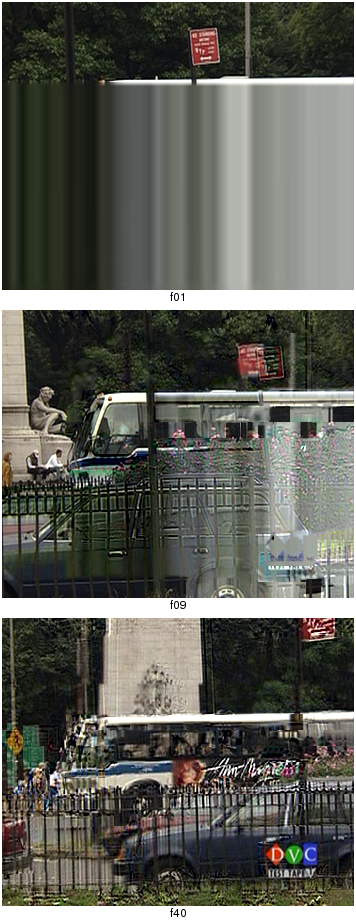
\includegraphics[width=0.9\textwidth]{./imgs/netsim.png}
	\caption{Ilustração do arquivo de configuração de descartes da ferramenta Netsim.}
	\label{fig:netsim}
	\fonte{Autoria Própria.}
\end{figure}

Neste caso, \emph{A} e \emph{C} indicam o número de entidades que atingem seu destino com sucesso e \emph{B} e \emph{D} indicam quantas serão descartadas. 
Sendo assim o streaming de vídeo da Figura \ref{fig:netsim}  teria seus primeiros \emph{A} pacotes intactos, seguidos de \emph{B} perdidos, mais \emph{C} pacotes intactos e ainda \emph{D} perdidos novamente.

\begin{table}[!h]
	\begin{tabular}{llll}
	./netsim & & \\
	& \texttt{--input} & \texttt{-i} & Define o caminho (absoluto ou relativo) e arquivo do vídeo \\ 
	& & & a ser processado pela simulação. \\
	& \texttt{--output} & \texttt{-o} & Define o caminho(absoluto ou relativo) e arquivo onde será \\ 
	& & & armazenado o vídeo resultante. \\
	& \texttt{--ts} & \texttt{-t} & (Opcional) Se presente, a entidade de descarte considerada \\
	& & & é um TS, caso contrário a unidade é um pacote UDP. \\
	& \texttt{--raffle} & \texttt{-r} & Indica o caminho (absoluto ou relativo) e arquivo a ser usado \\ 
	& & & como configuração de descartes. \\
	\end{tabular}
\end{table}


\subsection{Metric}
\label{des:metric}

A ferramenta Metric se trata da implementação de três métricas objetivas, as mesma encontradas na implementação do SASQV:

\begin{itemize}
	\item MSE
	\item PSNR
	\item MSSIM
\end{itemize}

Implementada em C++, também na forma de uma ferramenta \emph{stand-alone}, seu funcionamento é baseado em verificar disparidades entre dois vídeos fornecidos seguindo uma das métricas implementadas e fornecer um resultado numérico. 
Os vídeos a serem comparados devem possuir as mesmas dimensões e número de frames para serem passíveis de comparação. 
A ferramenta Metric pode receber os seguintes parametros:

\begin{table}[!h]
	\begin{tabular}{llll}
	& \texttt{--input} & \texttt{-i} & Define o caminho(absoluto ou relativo) e arquivo onde um dos \\ 
	& & & vídeos a serem comparados se encontra. \\
	& \texttt{--reference} & \texttt{-r} & Define o caminho(absoluto ou relativo) e arquivo onde o segundo \\
	& & & vídeo a ser comparado se encontra. \\
	& \texttt{--size} & \texttt{-s} & Define as dimensões (em pixels) dos vídeos a serem comparados. \\ 
	& & & Deve ser fornecida no formato 'largura'x'altura'. \\
	& \texttt{--metric} & \texttt{-m} & Define qual métrica será utilizada na comparação entre vídeos, \\
	& & & sendo uma string entre MSE, PSNR ou MSSIM. \\
	& \texttt{--window} & \texttt{-w} & Define qual o tamanho da janela (em pixels) a ser usado se \\ 
	& & & a métrica adotada for MSSIM. \\
	\end{tabular}
\end{table}

\section{Interface Gráfica}

A presente seção irá descrever com maiores detalhes as funcionalidades da interface gráfica desenvolvida para o SASQV2, separados conforme a finalidade de cada janela presente na mesma.

\subsection{Sessão}

A janela de Sessão consiste de um passo inicial de configuração --- onde se sucedem três telas conforme são fornecidos dados para a aplicação --- e um segundo passo onde é disparada uma sessão de avaliação subjetiva baseada na configuração fornecida préviamente.

A primeira tela se trata de configurações básicas da sessão, tal como um nome e descrição para facilitar a identificação como também a métrica a que será utilizada e o número de espectadores.
Na sequência é apresentada uma tela onde pode-se buscar e selecionar vídeos para serem exibidos na sessão de avaliação e for fim a tela para selecionar quais dispositivos remotos serão utilizados na avaliação. Ao final da configuração, pode-se dar início ao processo de avaliação subjetiva onde os vídeos selecionados serão então exibidos conforme a métrica selecionada.
Na Figura \ref{} pode-se observar o ambiente de exibição dos vídeos durante a avaliação.

%TODO colocar figura e corrigir referencia na linha acima

\subsection{Ferramentas}

Esta é a janela de maior complexidade no SASQV2, dado que nela se encontram os controles e opções que permitem usar todas as ferramentas descritas em \ref{des:ferramentas}. 
Por meio das abas presentes na parte superior da janela é possível acessar três telas diferentes: Gerador de Artefatos, Avaliador Objetivo e Gerador de Aleatoriedade. As funções específicas de cada uma delas são descritas a seguir:

\subsubsection{Gerador de Artefatos}

A tela do gerador de artefatos permite controlar de forma gráfica a execução e parametrização das ferramentas \emph{block}, \emph{blur} e \emph{netsim}. Nela pode-se observar três regiões distintas:

\begin{itemize}
	\item Uma lista de busca dos vídeos passíveis de degradação.
	\item Controladores específicos para cada ferramenta de degradação.
	\item Uma fila de tarefas de degradação a serem executadas.
\end{itemize}

Para adicionar um artefato em um vídeo é preciso selecionar um vídeo da lista e configurar uma das três ferramentas a disposição. 
Os parâmetros disponíveis na interface são condizentes com os parâmetros apresentados em \ref{des:ferramentas} para cada ferramenta.
Ao clicar no botão \emph{Adicionar}, uma tarefa com os detalhes do processo selecionado sera adicionada à lista na parte inferior da tela. É possível enfileirar quantas tarefas forem necessárias e então dar início ao processo de degradação dos vídeos clicando em iniciar.

\subsubsection{Avaliador Objetivo}

Nesta tela existem quatro componentes distintos que permitem configurar e utilizar a ferramenta \emph{metric} citada em \ref{des:metric}:

\begin{itemize}
	\item Uma lista de busca dos vídeos passíveis de avaliação.
	\item Uma lista de busca dos vídeos que podem ser tomados como referência.
	\item Um seletor de métricas objetivas dispiníveis.
	\item Uma fila de tarefas de avaliação a serem executadas.
\end{itemize}

Para efetuar uma avaliação objetiva é preciso selecionar dois vídeos a serem comparados, um como referência e outro como amostra, além da métrica desejada e clicar no botão \emph{Adicionar}.
Com isso, os vídeos e a métrica atualmente selecionados serão adicionados à lista de tarefas. 
Ao se clicar no botão \emph{Iniciar} todas as tarefas da lista serão processadas e uma janela de diálogo mostrará o valor resultante de cada avaliação, os quais também podem ser observados na janela de resultados descrita em \ref{des:resultados}.

\subsubsection{Gerador de Aleatoriedade}

Aqui é possível configurar e utilizar a ferramenta \emph{raffle} de \ref{des:raffle} por meio dos seguintes campos apresentados:

\begin{itemize}
	\item Nome do arquivo a ser gerado.
	\item Número de elementos a serem gerados.
	\item Quantidade de colunas no arquivo de saída.
	\item Tabela de configuraçaõ de distribuições estatísticas.
\end{itemize}



\subsection{Resultados}
\label{des:resultados}

\subsection{Configurações}
\subsection{Ajuda}

\section{Diagramas de Classes}

\section{Diagramas de Sequências}
\section{Considerações}
